\documentclass[fyp]{socreport}
\usepackage[utf8]{inputenc}
\usepackage[english]{babel}
\usepackage{charter}
\usepackage{fullpage}
\usepackage{hyperref}
\usepackage{amsmath}
\usepackage{booktabs}
\usepackage{graphicx}
\usepackage[backend=biber,sorting=none]{biblatex}
\addbibresource{socreport.bib}

\begin{document}
\pagenumbering{roman}
\projyear{2019/20}
\projnumber{H226080}
\author{Kuan Sheng Yuan, Jethro}
\title{Event-Driven Visual-Tactile Learning for Robots}
\advisor{Dr.\ Harold Soh}
\deliverables{
	\item Report: 1 Volume}
\maketitle

\begin{abstract}
  In this work, we contribute an event-driven visual-tactile perception system,
  built on spiking neural networks. Our perception system is trained, and tested
  end-to-end on novel multi-modal event-based data for two sensor modalities:
  (1) Tactile data, from our biologically-inspired fingertip tactile sensor,
  NeuTouch and (2) visual data, from the Prophesee camera. We evaluate our
  system on two robotic tasks: container classification, and slip detection. On
  both tasks, we observe good classification accuracies relative to standard
  deep learning methods. Our system can be run on neuromorphic hardware, making
  this a crucial first step towards enabling power-efficient, intelligent
  robots.

  \begin{keywords}
    Spiking Neural Networks, Multi-modal Machine Learning
  \end{keywords}

  \begin{implement} Python 3, PyTorch
  \end{implement}
\end{abstract}

% \listoffigures
% \listoftables
\tableofcontents

\chapter{Introduction\label{cha:intro}}

Human beings are blessed with innate abilities to integrate sensory information
from different stimuli. Our sense of smell, hearing, touch, vision, and taste
each contribute to how we perceive and act in the world. Consider the scenario
of fetching a carton of soy-milk from the fridge; humans use vision to locate
the carton, and are also able to infer from grasping the object, the amount of
soy-milk the carton contains. These actions (and inferences) are performed
robustly using a power-efficient neural substrate --- compared to popular deep
learning approaches for using multiple sensor modalities in artificial systems,
human brains require far less energy~\cite{li2016energyefficiency}.

In this work, we take crucial steps towards efficient visual-tactile perception
for robotic systems. We gain inspiration from biological systems, which are
\emph{asynchronous} and \emph{event-driven}. In contrast to resource-hungry deep
learning methods, event-driven perception offers an alternative approach that
promises power-efficiency and low-latency --- features that are ideal for
real-time mobile robots. However, event-driven systems remain under-developed
relative to standard synchronous perception methods~\cite{pfeiffer2018deep}.

We make multiple contributions that advance event-driven visual-tactile
perception. First, to enable richer tactile sensing, we use the NeuTouch
fingertip sensor. Compared to existing commercially-available tactile sensors,
NeuTouch's neuromorphic design enables scaling to larger number of taxels while
retaining low latencies.

Next, we investigate multi-modal (visual-tactile) learning using the NeuTouch
and the Prophesee event-based camera. Specifically, we develop a
\emph{visual-tactile spiking neural network} (VT-SNN) that incorporates both
sensory modalities for supervised-learning tasks. Different from conventional
deep artificial neural network (ANN) models, SNNs process discrete spikes
asynchronously, and thus, are arguably better suited to the event data generated
by our neuromorphic sensors. In addition, SNNs can be used on efficient
low-power neuromorphic chips such as the Intel Loihi~\cite{davies2018loihi}.

Our experiments center on two robot tasks: object classification and
(rotational) slip detection. In the former, we tasked the robot to determine the
type of container being handled and amount of liquid held within. The containers
were opaque with differing stiffness, and hence, both visual and tactile sensing
are relevant for accurate classification. We show that relatively small
differences in weight ($\approx 30$g across 20 object-weight classes) can be
distinguished by our prototype sensors and spiking models. Likewise, the slip
detection experiment indicates rotational slip can be accurately detected within
$0.08$s (visual-tactile spikes processed every $\approx 1$ms). In both
experiments, SNNs achieved competitive (and sometimes superior) performance
relative to ANNs with similar architecture.

The work presents an exciting opportunity to enable power-efficient intelligent
robots. Presented with labeled data, an event-driven perception network can be
trained end-to-end, and used on neuromorphic chips as robotic controllers.

\section{Research Outline}

In \autoref{cha:background}, we first provide a comprehensive study on SNNs. We
discuss why and when we should use spiking neural networks, and how to train
them. Crucially, we draw similarities between spiking neural networks and
recurrent neural networks, a recently discovered property that enables the
end-to-end training of these networks using gradient-based methods.

In \autoref{cha:vtsnn}, we contribute an event-driven visual-tactile
spiking-neural network (VT-SNN), which enables fast perception on two
event-based sensors: the NeuTouch~\cite{aiskinLee}, and the Prophesee event
camera. Here, we detail the experimental setups for the robotic tasks: object
classification and slippage detection. We discuss our experimental results, and
demonstrate that spiking neural networks achieve competitive (and sometimes
superior) performance over deep learning methods, and in addition having the
unique property of early classification.

This thesis was originally an exploratory project on spiking neural networks.
In the duration of this research, several different research directions have
been explored. In the chapters that follow, we discuss research directions we
have taken that were later abandoned.

In \autoref{cha:snnrl}, we evaluate the feasibility of spiking neural networks
as agents in a reinforcement learning setting. Reinforcement learning
environments are often temporal in nature, due to the interdependence between
states and actions in the environment. We hypothesised that spiking neural
agents were well suited in many reinforcement learning settings.

\section{Individual Contributions}
The event-driven visual-tactile perception system is a joint work between our
group, the Collaborative Learning \& Adaptive Robots (CLeAR) group, and the TEE
research group.

The TEE research group contributed the novel NeuTouch tactile sensor, which was
used to collect data for the tactile modality. The CLeAR group contributed: (1) a
visual-tactile spiking neural network (VT-SNN) that leverages multiple event
sensor modalities, (2) systematic experiments demonstrating the effectiveness of
our event-driven perception system on object classification and slip detection,
with comparisons to conventional ANN methods, and (3) visual-tactile event
sensor datasets comprising more than 50 different object classes across the
experiments, including RGB images and proprioceptive data from the robot.

Among the contributions of the CLeAR group, my individual contributions include
the experimentation (training and evaluation) of the VT-SNN models, as well as
some guidance on the ANN models. I am also looking into running these models on
neuromorphic hardware, to quantify the performance and power gains of using the
spiking models. During the research process, I also maintained the code
repository at high-quality. Model training was designed to be reproducible, and
parameter searches could be done efficiently across multiple GPUs. Different
experimental runs could also be plotted, and their results aggregated for later
analyses.

All work in subsequent chapters () % TODO
are my own.

\chapter{Background\label{cha:background}}

This chapter provides background knowledge about spiking neural networks. It
reviews the differences between deep neural networks, and spiking neural
networks (\ref{sec:gener-neur-netw}). It introduces the basics of spiking neural
networks (\ref{sec:spiking-neuron-model}), and its benefits
(\ref{sec:motiv-spik-neur}). Finally, we discuss how to train spiking neural
networks (\ref{sec:train-spik-neur}), and give some future directions.

\section{The Generations of Neural Networks\label{sec:gener-neur-netw}}

Neural network models can be classified into three generations, according to
their computational units: perceptrons, non-linear units, and spiking
neurons~\cite{MAASS19971659}. Perceptrons can be composed to produce a variety
of models, including Boltzmann machines and Hopfield networks. One
characteristic feature of perceptrons is that only give digital output.

Non-linear units apply an activation function with a continuous set of possible
output values to a weighted sum of the inputs. Classic examples of networks of
this second generation include feed-forward and recurrent sigmoidal neural
networks. These networks are able to compute functions with analog input and
output. Non-linear units are currently the most widely used computational unit,
and is responsible for the explosion of progress in machine learning research,
in particular, the success of deep learning. This is largely because networks
built with these units are trainable with well-researched gradient-based
methods, such as backpropagation.

Despite being biologically inspired, second-generation neural networks (ANNs)
bear little resemblance to the human cortex. In contrast to the digital
computation in ANNs, networks of neurons perform fast analog computations. This
inspired a the third generation of neural networks use computational units
called \emph{spiking neurons}, which communicate via discrete spikes. Much like
our biological neurons, spiking neurons are connected to each other at synapses,
receiving incoming signals at the dendrites, and sending spikes to other
downstream neurons via the axon. Each computational unit stores its membrane
potential, which fluctuates over time based on well-defined neuronal dynamics.
Rather than firing at each propagation cycle, these computational units fire
only when their individual membrane potentials crosses its firing threshold.

\begin{table}
  \centering
  \small
  \begin{tabular}{ l|ccc }
    \hline
    \hline
    \textbf{Name} & \textbf{Input} & \textbf{Output} & \textbf{Examples} \\
    \hline
    (1) Perceptrons & Digital & Digital & Hopfield Networks, Boltzmann Machines \\
    (2) Non-linear Units & Digital/Analog & Digital/Analog & Feed-forward \& Recurrent ANNs \\
    (3) Spiking Neurons & Analog & Analog & Feed-forward SNNs \\
    \hline
    \hline
  \end{tabular}
  \normalsize
  \caption{\label{tab:nn_generations} The three generations of neural networks. }
\end{table}

Henceforth, we shall term second-generation neural networks artificial neural
networks (ANNs), and third-generation neural networks spiking neural networks
(SNNs).

\section{Motivating Spiking Neural Networks\label{sec:motiv-spik-neur}}

Since ANNs have excellent performance, and can handle both digital and analog
input and output, why should we bother with spiking neural networks? In this
section, we motivate spiking neural networks from various perspectives.

\subsection{Information Encoding via Spikes}

To directly compare ANNs and SNNs, one can consider the real-valued outputs of
ANNs to be the firing rate of a spiking neuron in steady state. In fact, this
scheme, termed \emph{rate coding}, has been used to explain computational
processes in the brain~\cite{pfeiffer2018deep}.

However, experiments have shown that different actions are taken based on single
spikes~\cite{stemmler96_singl_spike_suffic}. In addition, the humans are capable
of performing tasks such as visual pattern analysis and pattern classification
in 100ms~\cite{thorpe2001spike}. Rate coding strategies are far too inefficient
for the rapid information transmission required for sensory processing. In
addition, the firing distribution of biological neurons is heavily skewed
towards lower firing rates. To obtain a good estimate of the firing rate, many
spikes would be required.

Different from ANNs, spiking neuron models are able to encode information beyond
the average firing rate: these models also utilize the relative timing between
spikes~\cite{guetig14_to_spike_or_when_to_spike}, or spike phases (in-phase or
out-of-phase). These time-dependent codes are termed \emph{temporal codes}, and
play an important role in biology. It has also been successfully demonstrated
that temporal coding achieves competitive empirical performance on
classification tasks for both generated datasets, as well as image datasets like
MNIST and CIFAR~\cite{comsa19_tempor_codin_spikin_neural_networ}.

There is additional benefit to encoding information directly in the temporal
domain. Architectures for atemporal artificial neural networks using a memory
mechanism, such as the LSTM, have been proposed. However, in these networks,
every neuron wait on the activation of all neurons in previous layers before
producing an answer. In spiking neural networks, the output layers spike over
time, and predictions can be made at any time-step. Hence, SNNs are able to
operate in two regimes. The first regime is a highly accurate but slow regime,
where predictions are made at later time-steps. This is the regime that
atemporal ANNs support, where predictions are typically made only after a fixed
time-step $T$. The second regime is a low accuracy but fast regime, where the
network fast predictions, at a much lower accuracy. This behaviour mirrors the
speed-accuracy tradeoff observed in human
decision-making~\cite{comsa19_tempor_codin_spikin_neural_networ}, and we also
observe and exploit this property in our work described in~\autoref{cha:vtsnn}.

By observing that biological neurons use spikes to communicate information, a
wide range of coding schemes have been developed. Each of these codes have
different information capacities, and their pros and cons. We defer this
discussion to~\cite{thorpe2001spike}, but summarize the coding schemes
in~\autoref{tab:coding_schemes}. Spiking neural networks are able to take
advantage of these various coding schemes.

\begin{table}
  \centering
  \small
  \begin{tabular}{l|c}
    \hline
    \hline
    \textbf{Coding Scheme} & \textbf{Encoding of Information} \\
    Rate Coding & Firing rate of neurons \\
    Count Code & Count of number of neurons that spike during in time window \\
    Binary Code & Binary pattern of length $N$ from $N$ neurons (e.g. $0010$,
                  where the third neuron spiked) \\
    Temporal Code & Time of each spike in the spike
                    train \\
    Rank Code & Order in which neurons fire \\
    Synchrony Code & Patterns from a population of neurons \\
    \hline
    \hline
  \end{tabular}
  \normalsize
  \caption{Coding Schemes in Spiking Neural Networks}
  \label{tab:coding_schemes}
\end{table}

\subsection{Practical Benefits}

\subsubsection{Real-time Performance and Parallelism}
The ability to communicate information in a small number of spikes has immense
practical benefit.

First, the analog communication modeled in spiking neurons allow for naturally
parallel and high-speed computation. The promise of real-time performance is a
key motivator behind the development of neuromorphic hardware. Typical hardware
such as the everyday computer uses the von Neumann architecture, which separates
memory and processing, which has severe implications on performance.
Neuromorphic hardware collocates memory and processing, overcoming the von
Neumann bottleneck~\cite{Backus_1978}.

\subsubsection{Power Efficiency}
Next, the primary motivation cited in present-day literature is the
power-efficiency of spiking neural networks. First, less energy is used in
propagating fewer spikes. Second, communication via spikes is much more
computationally efficient than the floating point arithmetic performed in
artificial neural networks. This low energy footprint is a highly desirable
trait in robotics applications.

\subsubsection{Biological Plausibility\label{bioplausible}}
A faction of the machine learning and neurobiology community strives for
emulation of the biological brain. There are several incompatibilities between
ANNs and the current state of neurobiology that are not easily reconciliated.

First, neurons in ANNs communicate via continuous-valued activations.  This is
contrary to neurobiological research, which shows that communication between
biological neurons communicate by broadcasting spike trains: trains of action
potentials to downstream neurons. The spikes are to a first-order approximation
of uniform amplitude, unlike the continuous-valued activations of ANNs.

Second, backpropagation as a learning procedure also presents incompatibilities
with the biological brain~\cite{TAVANAEI201947}. Consider the chain rule in
backpropagation:

\begin{equation}
  \label{chainrule}
  \delta_{j}^{\mu}=g^{\prime}\left(a_{j}^{\mu}\right) \sum_{k} w_{k j} \delta_{k}^{\mu}
\end{equation}

\(\delta_{j}^{\mu}\) and \(\delta_{k}^{\mu}\) denote the partial derivatives of
the cost function for input pattern \(\mu\) with respect to the net input to
some arbitrary unit \(j\) or \(k\). Unit \(j\) projects feed-forward connections
to the set of units indexed by \(k\). \(g(\cdot)\) is the activation function
applied to the net input of unit \(j\), denoted \(a_j^{\mu}\), \(w_{kj}\) are
the feedforward weights projecting from unit \(j\) to the set of units indexed
by \(k\).

The chain rule formulation presents two problems. First, the gradients
\(g'(\cdot)\) requires derivatives, but \(g(\cdot)\) in spiking neurons is
represented by sum of Dirac delta functions, for which derivatives do not
exist. Second, the expression \(\sum_{k} w_{k j} \delta_{k}^{\mu}\) uses
feedforward weights in a feedback fashion. This mean that backpropagation is
only possible in the presence of symmetric feedback weights, but these do not
exist in the brain. In addition, during backpropagation the error assignment for
each neuron is computed using non-local information.

\subsubsection{Online Learning and Fault Tolerance}

Biological neurons brain evolve and adapt as time passes, creating new
connections, and destroying old ones. While the phenomenon of
\emph{neuroplasticity} is not yet well understood, it is hoped that the learning
mechanisms behind human intelligence will inspire a new generation of online
learning algorithms.

Neurons also frequently perish, and the human brain has the ability to
self-heal. In the same way, spiking neural network architectures can be designed
to possess the same self-healing and fault tolerance characteristics. This is a
desirable trait for systems where uptime is critical.

In conclusion, the main motivations for spiking neural networks are the
following:

\begin{itemize}
  \item Neuromorphic hardware can overcome the von Neumann bottleneck
  \item When combined with neuromorphic hardware, SNNs can:
  \begin{itemize}
    \item achieve real-time performance via asynchronous spiking communication
    \item achieve low power consumption from sparse spiking computation
    \item implement plasticity-inspired online learning mechanisms
    \item Fault tolerance beyond what von Neumann architectures can provide
  \end{itemize}
  \item Some SNNs have biologically-plausible neuron models, which can help
  answer open questions in neuroscience
\end{itemize}

\section{A Spiking Neuron Model\label{sec:spiking-neuron-model}}
In spiking neural networks, neurons exchange information via spikes, and the
information received depends on:

\begin{description}
\item[{Firing frequencies}] The relative timing of pre and post-synaptic spikes,
and neuronal firing patterns
\item[{Identity of synapses used}] Which neurons are connected, whether their
synapses are inhibitory or excitatory, and synaptic strength
\end{description}

Each neuron has a corresponding model that encapsulates its state: the current
membrane potential. As with the mammalian brain, incoming spikes increase the
value of membrane potential. The membrane potential eventually decays to resting
potential in the absence of spikes. These dynamics are often captured via
first-order differential equations. Here we define the Spike Response Model
(SRM), a simple but widely-used model describing the momentary value of a neuron
\(i\).

We define for presynaptic neuron \(j\),
\(\epsilon_{ij}(t) = u_{i}(t) - u_{\text{rest}}\). For a few input spikes, the
membrane potential responds roughly linearly to the input spikes:

\begin{equation} u_i{t} = \sum_{j}\sum_{f} \epsilon_{ij}(t - t_j^{(f)}) + u_{\text{rest}}
\end{equation}

SRM describes the membrane potential of neuron \(i\) as:

\begin{equation} u_i{t} = \eta (t - \hat{t_i}) + \sum_{j}\sum_{f} \epsilon_{ij}(t - t_j^{(f)}) + u_{\text{rest}}
\end{equation}

where \(\hat{t_i}\) is the last firing time of neuron \(i\).

We refer to moment when a given neuron emits an action potential as the firing
time of that neuron. We denote the firing times of neuron \(i\) by \(t_i^{(f)}\)
where \(f = 1,2,\dots\) is the label of the spike.  Then we formally denote the
spike train of a neuron \(i\) as the sequence of firing times:

\begin{equation} S_i(t) = \sum_{f} \delta\left( t - t_i^{(f)} \right)
\end{equation}

where \(\delta(x)\) is the Dirac-delta function with \(\delta(x) = 0\) for
\(x \ne 0\) and \(\int_{-\infty}^{\infty} \delta(x)dx = 1\). Spikes are thus
reduced to points in time.


\subsection{Neuromorphic Hardware\label{neuromorphic}}

In a traditional Von Neumann architecture, the logic core operates on data
fetched sequentially from memory. In contrast, in neuromorphic chips both
computation and memory are distributed across computational units that are
connected via synapses. The neuronal architecture and parameters hence play a
key role in information representation and define the computations that are
performed.

It has also been observed that spike-trains in the mammalian brain are often
sparse in time, suggesting that timing and relative timings of spikes encode
large amounts of information. Neuromorphic chips implement this same sparse,
low-precision communication protocol between neurons on the chip, and by
offering the same asynchronous, event-based parallelism paradigm that the brain
uses, are able to perform certain workloads with much less power than Von
Neumann chips.

These integrated circuits are typically programmed with spiking neural
networks. Examples of such chips include IBM's TrueNorth~\cite{Merolla668} and
Intel's Loihi~\cite{davies2018loihi}. Because spiking neural networks have not
yet been successfully trained on many tasks, neuromorphic chips has seen little
practical use. These chips have only recently been successfully used in robotic
navigation~\cite{SnnSlam}, and solving graph problems by manual construction of
the network graph~\cite{Severa2016SpikingNA}.

\section{Training Spiking Neural Networks\label{sec:train-spik-neur}}

As explained in \autoref{neuromorphic}, it is desirable to train spiking neural
networks to perform arbitrary tasks, utilizing power-efficient neuromorphic
chips that break the Von Neumann bottleneck. We classify the training strategies
by their usage of gradients, and discuss certain optimization techniques.

\subsection{Non-gradient based methods}

Spiking neurons communicate via spikes, hence, unlike ANNs, gradients are
non-existent. In addition, backpropagation is not biologically plausible (see
\autoref{bioplausible}). This motivates the use of plasticity-based methods and
evolutionary strategies for training SNNs.

One category of learning rules used in SNNs are local learning rules.  These
rules include Hebbian learning (neurons that fire together wire together), and
its extension: the spike-timing-dependent-plasticity rule (STDP). Inspired by
experiments in neuroscience, central to these learning rules is the theme that
neuron spike ordering and their relative timings encode information. STDP
adjusts the strength of connections between neurons using the relative timing of
a neuron's output and its input potentials (hence, spike-timing dependent).

In machine learning terminology, the weights of the synapses are adjusted
according to fixed rules for each training example. Each synapse is given a
weight \(0 \le w \le w_{\max}\), characterizing its strength, and its change
depends on the exact moments \(t_{pre}\) of pre-synaptic spikes and \(t_{post}\)
of post-synaptic spikes~\cite{sboev18_spikin_neural_networ_reinf_learn}:

\begin{equation} \Delta w=\left\{\begin{array}{l}{-\alpha \lambda \cdot \exp \left(-\frac{t_{\mathrm{pre}}-t_{\mathrm{post}}}{\tau_{-}}\right), \text {if } t_{\mathrm{pre}}-t_{\mathrm{post}}>0} \\ {\lambda \cdot \exp \left(-\frac{t_{\mathrm{post}}-t_{\mathrm{pre}}}{\tau_{+}}\right), \text {if } t_{\mathrm{pre}}-t_{\mathrm{post}}<0}\end{array}\right.
\end{equation}

where \(\tau_{+}\) and \(\tau_{-}\) are time constants. \(\tau_{+} = 16.8ms\)
and \(\tau_{-} = 33.7ms\) are reasonable approximations obtained experimentally.

There are several libraries like BindsNET~\cite{10.3389/fninf.2018.00089} that
simulate SNNs on Von Neumann computers implementing these rules. Recent attempts
have been made to combine Reinforcement Learning and STDP:\@ both in solving RL
problems~\cite{10.3389/fninf.2018.00089}, and using the reinforcement learning
framework to train
SNN~\cite{10.3389/fnbot.2019.00018,10.3389/fnins.2018.00435}. However, SNNs
trained using the STDP learning rule have yet to achieve comparable performance
compared to ANNs on relatively simple datasets like MNIST~\cite{TAVANAEI201947}.

\subsection{Gradient-based methods}

Performance is important for practical applications, and gradient-based training
methods such as backpropagation has shown competitive performance. It is thus
desirable to train spiking neural networks with these gradient-based methods.

There are several problems with spike-compatible gradient-based methods. First,
most of these methods cannot train neurons in the hidden layers: they can only
train neurons at the final layer, that receive the desired target output
pattern~\cite{urbanczik09_gradien_learn_rule_tempot,training_deep_snn_bpp_lee}.
Second, the discontinuous, binary nature of spiking output needs to be
addressed. For example, SpikeProp approximates the membrane threshold function
at a local area with a linear function, introducing gradients and computing the
exact formulae for error backpropagation for synaptic weights and spike
times~\cite{spikeprop}. Others have modified the threshold function with a gate
function~\cite{NIPS2018_7417}, used the alpha transfer function to derive
gradient update rules~\cite{comsa19_tempor_codin_spikin_neural_networ}, and
approximate the dirac-delta spikes with a probability density
function~\cite{NIPS2018_7415}.

Another approach is converting trained ANN models into
SNNs~\cite{rueckauer16_theor_tools_conver_analog_to}. Common ANN layers such as
softmax, batch normalization and max-pooling layers have their corresponding
spiking counterparts.

Equilibrium Propagation was recently proposed to solve the neurobiological
incompatibilities of backpropagation~\cite{10.3389/fncom.2017.00024}. Because
the gradients are defined only in terms of local perturbations, the synaptic
updates correspond to the standard form of STDP.\@ The propagated signal encodes
the gradients of a well-defined objective function on energy-based models, where
the goal is to minimize the energy of the model. To resolve the issue of
communication using binary-valued signals, step-size annealing was used to train
spiking neural networks with Equilibrium Propagation
~\cite{pmlr-v89-o-connor19a}.

\subsection{Future Research Areas\label{sec:future-rese-areas}}

A nascent area is local learning on neuromorphic chips. Thus far spiking neural
networks are simulated and trained before deployment on a neuromorphic chip. In
Intel's Loihi chip, each core contains a learning engine that can update
synaptic weights using the 4-bit microcode-programmed learning rules that are
associated with that synapse. This opens up areas for online learning.

\chapter{Event-driven Visual-Tactile Sensing and Learning for Robots\label{cha:vtsnn}}

In the introduction, we have alluded to VT-SNN, an event-driven
visual-tactile perception system using spiking neural networks. This chapter
describes the work done on that project. In \autoref{sec:snnrl_related}, we
discuss the prior art for visual-tactile systems. In \autoref{sec:snnrl_vtsnn},
we discuss model architecture and model training. In
\autoref{sec:snnrl_exp_setup}, we detail the robot hardware setup used across
our experiments. Next, we discuss our experimental methods and results for our
two robotics tasks: container classification
(\autoref{sec:snnrl_container_class}), and slippage detection
(\autoref{sec:snnrl_slippage}). We run the trained models on the Intel Loihi
in~\autoref{sec:snnrl_neuromorphic} to quantify the gains in power-efficiency
and inference speeds. Finally, we conclude our work
(\autoref{sec:snnrl_conclusion}), and provide future research directions
(\autoref{sec:snnrl_future_work}).

This work has been submitted to ROS 2020.

\section{Related Work\label{sec:snnrl_related}}

In this section, we give an overview of related work on visual-tactile perception for robotics. Much of the work on event-based perception has been covered in~\autoref{cha:background}, and will not be repeated here.

\subsection{Visual-Tactile Perception for Robots}

% To this end, we have seen advancements in both tactile sensing and computer
% vision, using deep neural networks (DNNs). Different types of tactile sensors
% have been used in robotic manipulation in slippage
% detection~\cite{meier2016tactile} and tactile object
% recognition~\cite{gao2016deep}. Convolutional neural networks (CNNs) have also
% become commonplace in vision tasks, such as image segmentation, and object
% recognition. Deep reinforcement learning has also been successfully used for
% learn agents that are successful in performing robotic tasks, using vision
% data~\cite{levine2017handeye}. The remarkable success of deep learning can be
% attributed to advancements in gradient-based training methods and model
% architectures, allowing larger and deeper models to be trained and deployed.

\section{Visual-Tactile Spiking Neural Network (VT-SNN)\label{sec:snnrl_vtsnn}}

\section{Robot and Sensors Setup\label{sec:snnrl_exp_setup}}

\section{Container \& Weight Classification\label{sec:snnrl_container_class}}

\section{Rotational Slippage Classification\label{sec:snnrl_slippage}}

\section{Gains on Neuromorphic Hardware\label{sec:snnrl_neuromorphic}}

\section{Conclusion\label{sec:snnrl_conclusion}}

\section{Future work\label{sec:snnrl_future_work}}

\chapter{Reinforcement learning in Spiking Neural Networks\label{cha:snnrl}}

% TODO Introduction
% TODO RL survey

\subsection{The Cartpole Environment}


We use the Cartpole-v0 environment, a popular environment provided by
OpenAI.\@ The official description is as follows~\cite{openai_gym}:

\begin{quote} A pole is attached by an un-actuated joint to a cart, which moves
along a frictionless track. The system is controlled by applying a force of +1
or -1 to the cart. The pendulum starts upright, and the goal is to prevent it
from falling over. A reward of +1 is provided for every time-step that the pole
remains upright. The episode ends when the pole is more than 15 degrees from
vertical, or the cart moves more than 2.4 units from the center.

CartPole-v0 defines ``solving'' as getting average reward of 195.0 over 100
consecutive trials.
\end{quote}

\begin{figure}[htbp] \centering
  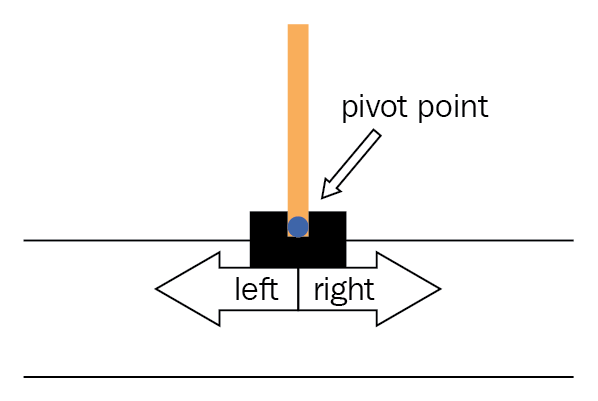
\includegraphics[width=.9\linewidth]{images/openai_gym.png}
  \caption{The OpenAI CartPole environment}
\end{figure}

\subsection{Training a Simple ANN agent}

First, we attempt to solve the problem with a simple MLP ANN agent that takes in
the four observations, and outputs as logits the probability of each action. The
action is then sampled from a 2-outcome categorical distribution with the logits
as the outcome probabilities. We do this so we can compare the performance of
the policies, learnt under the same conditions (learning rule, environment
parameters etc.).

Since SLAYER uses PyTorch, we implement vanilla policy gradients in PyTorch to
train the MLP agent. We use Sacred~\cite{klaus_greff-proc-scipy-2017} to log and
ensure reproducibility of our experiments.\footnote{This repository is hosted on
Github at \url{https://github.com/jethrokuan/snnrl/}. The repository is private,
request access as required.}

Experiments show that the ANN model learns to solve the environment quickly when
trained with VPG, as shown in \autoref{fig:vpg_mlp}. The agent obtains an
average episodic return of 200, ``solving'' the environment at 2000 time-steps.

\begin{figure}[htbp] \centering
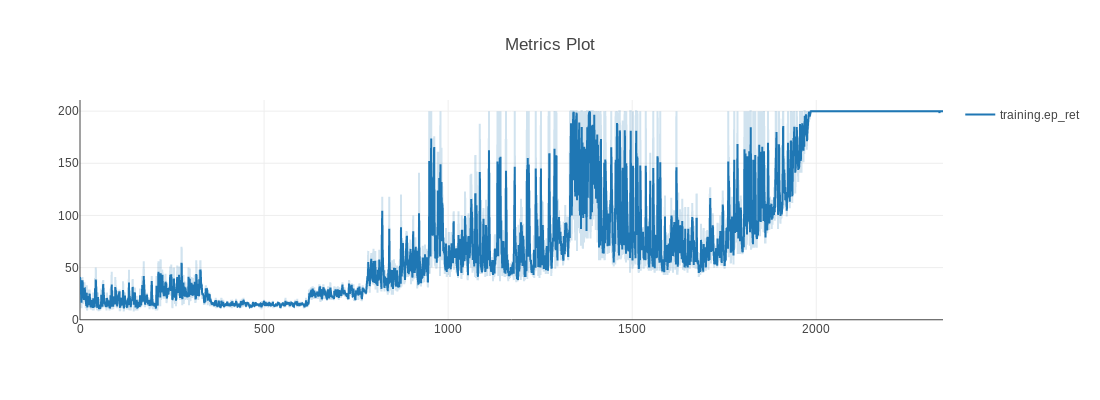
\includegraphics[width=.9\linewidth]{images/vpg_mlp.png}
\caption{\label{fig:vpg_mlp} Plot of average episode returns over time-steps for
a simple MLP agent.}
\end{figure}

\subsection{Training a SNN agent}

Similarly, we attempt to train the SLAYER model to solve the CartPole-v0. Each
SLAYER layer takes in a spike train as input and produces a spike train as
output. The objective function for supervised learning tasks such as
classification is defined in the paper, and is similar to
cross-entropy~\cite{NIPS2018_7415}.

Since the input to the Slayer model are spike trains, we require an encoder
mapping the environment observations into the fixed-length spike trains that
SLAYER accepts,as shown in \autoref{fig:slayer_rl}.

\begin{figure}[htbp] \centering
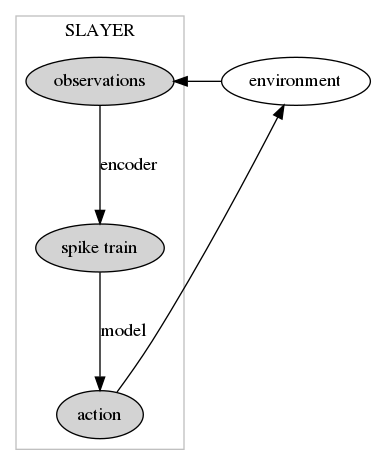
\includegraphics[height=7cm]{images/snn_encode.png}
\caption{\label{fig:slayer_rl} The SLAYER model requires an additional encoder
to transform the observations into spike trains as input.}
\end{figure}

We encode the observations by modelling the observations as Poisson
processes~\cite{heeger2000poisson}. First, we convert each of the four
observations into 2 non-negative observations: their absolute value, and their
sign. A negative value has an observation value of 0, and a positive value has
observation value of 1. We divide time into short, discrete intervals
\(\delta t\), and generate a sequence of random numbers \(x[i]\) uniformly
between 0 and 1. For each interval, if \(x[i] \le r \delta t\), generate a
spike. We produce spike trains of 300 time-steps as input to the SLAYER model
from the 8 observation values (scaled appropriately).

As shown in \autoref{fig:snn_vpg}, the SLAYER model fails to learn to solve the
problem.

\begin{figure}[htbp] \centering
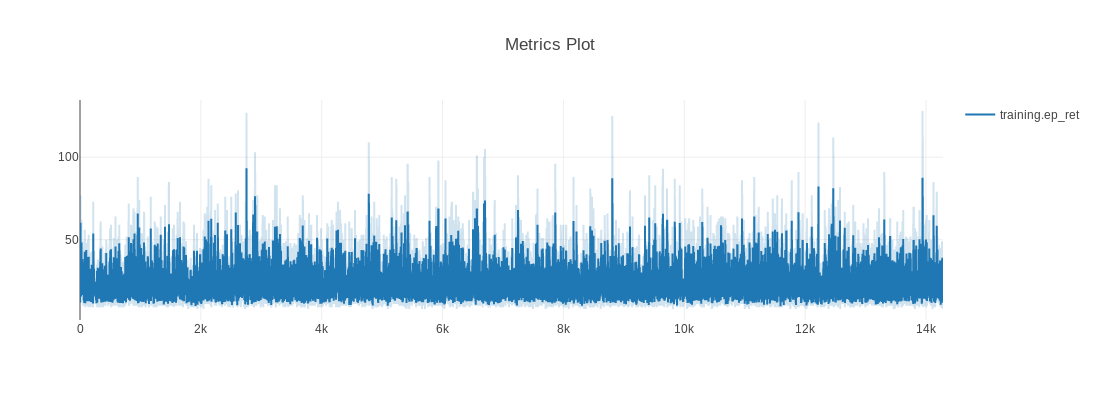
\includegraphics[width=.9\linewidth]{images/slayer_poisson.png}
\caption{\label{fig:snn_vpg} The SLAYER model with a Poisson encoder for the
observations fails to learn to solve the problem.}
\end{figure}

The problem likely resides in way encoding is done. The domain of the value of
some observations in the Cartpole environment is the range over all real
numbers, and encoding values over the entire range of real numbers is
tricky. There is no linear mapping, and changes in observation values may not
result in changes of noticeable magnitude in the mapped value.

There has, however, been works on encoding images into spike trains.  This is
particularly common as many spiking neural architectures are evaluated on a
converted MNIST image dataset. Hence, we move towards training spiking neural
networks on image observations.

\subsection{The ImageCartpole Environment}

To bypass the encoding issue described earlier, we turn towards training agents
on the pixels of the environment. We create a Cartpole environment such that the
observation is the difference in pixels of the current frame and the previous
frame. We term this modified environment ImageCartpole.

We train a simple CNN on this environment, using VPG.\@ Training this agent takes
significantly more time, as seen in \autoref{fig:imagecartpole_cnn}. However,
the agent is still able to learn from the observations, suggesting that this
environment is solvable by a SNN agent.

\begin{figure}[htbp] \centering
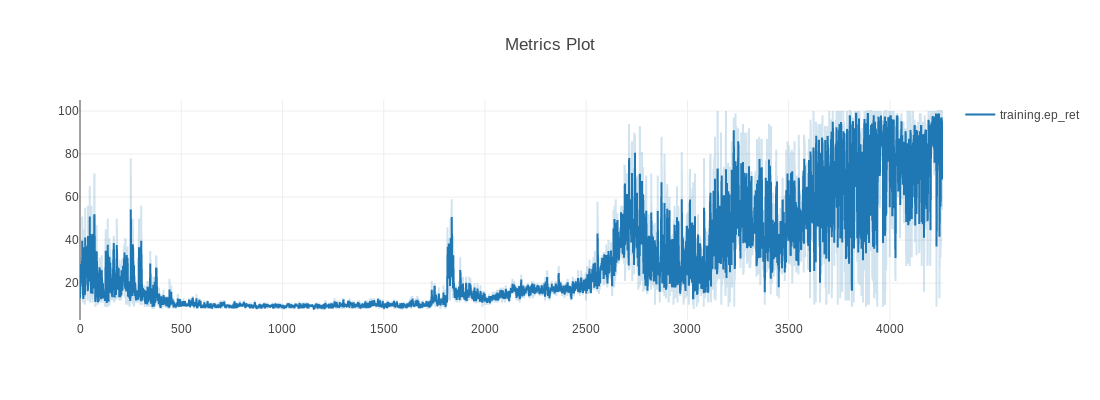
\includegraphics[width=.9\linewidth]{images/imagecartpole_cnn.png}
\caption{\label{fig:imagecartpole_cnn} Plot of the average episode return of a
CNN agent on the ImageCartpole environment over time.}
\end{figure}

At the time of submission, the SNN agent is unable to learn a good policy, but
more engineering work is required before any conclusions can be made.

\section{Future Work}

It is hoped that the SLAYER model is able to learn to solve simple environments
such as the Cartpole environment. Once it is established that gradient-based RL
methods also work for training SLAYER, we would move on towards milestones 3 and
4. If we are unable to learn a good policy via existing reinforcement learning
methods, some exploration into tweaking the learning rules or spiking neural
architecture is warranted.

As a closing thought, the way the cartpole environment is currently being used
also does not fully utilize the power of spiking neural networks. At each
time-step, observations are converted to full spike trains. SNNs are often able
to make predictions based on early spikes, albeit less reliable. This is not
exploited in the current environment formulation, where a full spike train of
fixed length is received before an action is taken.

In my idealized formulation of RL environment for SNNs, the following should be
satisfied:

\begin{enumerate}
  \item The action space should contain a no-op: in the case of the cartpole
  environment, this is as simple as adding the action of not applying force to
  the cart, instead of choosing between left or right
\item At each observation, the observation should be spikes, rather than spike
trains
\end{enumerate}

The SNN agent receives spikes at each time-step, and after gaining enough
confidence to take an action, it takes the action at that time-step. I
hypothesize that SNN agents should be able to solve such environments, by
exploiting the temporal information encoded in the relative timing between
spikes (in this case, number of timesteps) and that each spiking neuron stores
such temporal state, without the use of recurrent networks or replay buffers
common in current ANN setups.

\printbibliography

\appendix
\end{document}
